\chapter{Implementierung und Evaluation}
\label{ch:evaluation}

Zunächst beschreibt \autoref{sec:implementierung} die Implementierung des Prototyps zur Videoaufzeichnung mit den entsprechenden Frameworks.
Alle Prototypen stehen unter \url{https://github.com/lukaspanni/cross-platform-evaluation} unter der MIT-Lizenz zur Verfügung.
Dabei wird erläutert, wie die einzelnen Komponenten des Prototyps implementiert werden und welche zusätzlichen Komponenten eingesetzt werden müssen, um die geforderte Funktionalität umzusetzen.
Die Frameworks verwenden verschiedene Bezeichnungen für eingebundene Komponenten von Drittanbietern.
Zur einheitlichen Beschreibung werden diese in den folgenden Abschnitten jeweils als Plugins bezeichnet.
Außerdem wird jeweils beschrieben, inwiefern die geforderte Grundfunktionalität umgesetzt werden kann und welche Einschränkungen, zum Beispiel bei der Einstellung der Parameter, existieren.
In \autoref{sec:evaluation_allgemein} werden anschließend die Ergebnisse der allgemeinen Evaluationen nach den, in \autoref{sec:kriterien} beschriebenen Kriterien, zusammengefasst.


\section{Implementierung und Evaluation der Grundfunktionalität}
\label{sec:implementierung}

Insgesamt ist festzustellen, dass die Grundfunktionalität der Videoaufzeichnung mit allen untersuchten Frameworks mit vorhandenen Plugins umgesetzt werden kann.
Welche Komponenten verwendet wurden, welche Probleme aufgetreten sind und welche Einstellmöglichkeiten für die Parameter bestehen ist in den Abschnitten \ref{sec:evaluation_flutter} bis \ref{sec:evaluation_reactnative} beschrieben.
Auch der Zugriff auf den Gerätespeicher zur Speicherung der Videos ist in allen Frameworks möglich.
Dabei ist jedoch aufgefallen, dass kein Framework plattformübergreifende Speicherpfade unterstützt.
Stattdessen muss für jede Plattform ein passender Pfad, angepasst an die jeweilige Dateisystemstruktur, erzeugt werden.
Erste Unterschiede zeigen sich bei der Wiedergabe aufgezeichneter Videos.
Diese ist in Ionic mit Cordova mit allen getesteten Plugins nicht möglich.


\subsection{Implementierung mit Flutter}
\label{sec:evaluation_flutter}

Für den Zugriff auf Kamerafunktionen steht ein offizielles Dart Package beziehungsweise Plugin zur Verfügung \cite{Dart_Camera}.
Über dieses Plugin ist die Aufzeichnung von Videos unter Android und iOS möglich und einige Parameter können angepasst werden.
Für die Speicherung ist kein zusätzliches Plugin notwendig, der Zugriff auf Gerätespeicher ist in Flutter bereits integriert.
Zur Wiedergabe der Videos wird das offizielle Video-Player-Plugin verwendet \cite{Dart_Video}.

Die erforderlichen Anforderungen, sowie die Wiedergabe von Videos, können somit mit Flutter vollständig umgesetzt werden.
Allerdings gibt es einige Einschränkungen bei den einstellbaren Parametern.
So sind weder Belichtungszeit noch ISO-Wert einstellbar, für die Belichtung kann nur ein bestimmtes Offset für ein allgemein helleres beziehungsweise dunkleres Video gesetzt werden.
Zudem kann die Aktualisierung der automatischen Belichtungssteuerung gestoppt werden, die letzte automatische Einstellung bleibt dabei erhalten.
Der Fokus kann ebenfalls nicht komplett manuell gewählt werden, stattdessen kann ein Punkt auf dem Bildschirm ausgewählt werden, welcher vom Autofokussystem als Ausgangspunkt verwendet wird.
Für das Bildformat stehen bis zu fünf verschiedene Voreinstellungen zur Verfügung, wobei die Verfügbarkeit vom verwendeten Gerät abhängt.
Weißabgleich, Videocodec und Bildrate lassen sich ebenfalls nicht einstellen.
Außerdem konnte nicht jeder verfügbare Sensor des Android-Testsmartphones ausgewählt werden.


\subsection{Implementierung mit Ionic und Cordova}
\label{sec:evaluation_ionic}

Allgemein erlaubt Cordova den Zugriff auf native Funktionen, wie die Videoaufzeichnung nur über Plugins.
Erste Quelle für bestehende Plugins ist bei Verwendung von Ionic als UI-Toolkit die Sammlung offiziell unterstützter und getesteter Plugins, die unter \url{https://ionicframework.com/docs/native/} bereitsteht.
Hier konnten drei Plugins identifiziert werden, welche den Zugriff auf Kamerafunktionen ermöglichen.
Das naheliegende Plugin \textit{cordova-plugin-camera} erlaubt nur die Aufzeichnung von Bildern \cite{Cordova_Camera}.
Das Plugin \textit{cordova-plugin-camera-preview} ermöglicht zwar die Aufzeichnung von Videos, jedoch ist diese Funktion nur auf Android-Geräten verfügbar \cite{Cordova_CameraPreview}.
Lediglich das Plugin \textit{cordova-plugin-media-capture} erlaubt die Aufzeichnung von Videos auf allen Plattformen \cite{Cordova_MediaCapture}.
Jedoch verwendet dieses Plugin eine vom Betriebssystem bereitgestellte Aufzeichnungsfunktion, sodass aus der App heraus nur das Videoaufzeichnungsfenster geöffnet werden kann.
Dabei sind keinerlei Einstellungen der in \autoref{tab:parameter_support} aufgeführten Parameter möglich.
Auch außerhalb der offiziellen Sammlung von verifizierten Plugins konnten keine Plugins identifiziert werden, welche die Einstellung einiger Parameter unterstützen.
Die Speicherung aufgezeichneter Videos erfolgt ohne zu erkennende Einschränkungen über das offizielle Plugin \textit{cordova-plugin-file} \cite{Cordova_File}.
Die Wiedergabe der Videos hingegen konnte weder über das HTML-Video Element noch durch ein Plugin realisiert werden. 

Damit sind die erforderlichen Anforderungen zwar umgesetzt, jedoch werden keine der optionalen Anforderungen erfüllt.
Um die optionalen Anforderungen umzusetzen, müssten spezifische Plugins implementiert werden.
Dementsprechend ist die Implementierung einer Videoaufzeichnungsanwendung mit Ionic und Cordova nur stark eingeschränkt möglich.


\subsection{Implementierung mit Xamarin}
\label{sec:evaluation_xamarin}

Da Xamarin prinzipiell die Nutzung der nativen \acp{API} unterstützt, sind theoretisch alle Kamerafunktionen nutzbar.
Allerdings sollen im Rahmen dieser Arbeit nur die vorhandenen plattformübergreifenden Abstraktionen des Frameworks genutzt werden.
Die offizielle Bibliothek \textit{Xamarin.Essentials} ermöglicht neben der Nutzung weiterer nativer Funktionen auch den Zugriff auf verschiedene Kamerafunktionen.
Zum Zugriff auf die Kamera steht eine stark vereinfachte \ac{API} über die statische Klasse \textit{MediaPicker} bereit \cite{Xamarin_MediaPicker}.
Wie das, in der Implementierung mit Cordova eingesetzte Plugin, wird auch hier die Aufzeichnung von Videos über die vom Betriebssystem bereitgestellte Aufzeichnungsfunktion realisiert.
Deshalb ist auch hier die Aufzeichnung von Videos zwar möglich, jedoch können keine Parameter aus der Anwendung heraus gesetzt werden.
Der Zugriff auf den Gerätespeicher ist wie bei Flutter ohne zusätzliche Abhängigkeiten möglich.
Die Wiedergabe der Videos ist über ein entsprechendes \ac{UI}-Element der offiziellen Bibliothek \textit{XamarinCommunityToolkit} \cite{Xamarin_CommunityToolkit} ohne Einschränkungen möglich.

Mit Xamarin lassen sich ohne die direkte Verwendung nativer \acp{API} nur die erforderlichen Anforderungen uneingeschränkt erfüllen.
Auch die Wiedergabe der Videos ist ohne Einschränkungen möglich.
Die optionale Einstellbarkeit der Parameter kann hingegen nicht umgesetzt werden.


\subsection{Implementierung mit React Native}
\label{sec:evaluation_reactnative}

Für die Videoaufzeichnung mit React Native konnten zwei geeignete Native Modules beziehungsweise Plugins identifiziert werden.
Da das Plugin \textit{react-native-vision-camera} \cite{Vision_Camera} bei der Einstellung von Parametern mehr Flexibilität bietet als das Pluguin \textit{expo-camera} \cite{Expo_Camera}, wird für die prototypische Implementierung dieses Plugin verwendet.
Für Speicherung und Wiedergabe der Videos müssen zusätzlich \textit{react-native-fs} \cite{ReactNative_FileSystem} respektive \textit{react-native-video} \cite{ReactNative_Video} eingebunden werden.
Das Plugin \textit{react-native-vision-camera} ist auf die neue Architektur von React Native ausgelegt, welche bei neuen Projekten standardmäßig aktiviert ist.
Ebenfalls standardmäßig aktiviert ist die Verwendung der JavaScript Engine Hermes.
Diese Einstellungen werden für die Implementierung beibehalten.

Die erforderlichen Anforderungen und die Wiedergabe von Videos können mit React Native ohne Einschränkungen umgesetzt werden.
Bei der Einstellbarkeit der Parameter gibt es im Vergleich mit den anderen Frameworks zudem weniger Einschränkungen.
So ist eine freie Wahl des Sensors möglich, auf Basis derer die weiteren Einstellmöglichkeiten abhängig von den Fähigkeiten des Sensors eingeschränkt werden.
Verschiedene Sensoren unterstützen dabei unterschiedliche Kombinationen von Einstellungen, welche als sogenannte Formate abgerufen werden können.
Das Format definiert insbesondere die Auflösung und den Farbraum.
Abhängig vom Format kann die Bildrate für Videoaufnahmen in einem, im Format angegebenen, Bereich eingestellt werden.
Bei den Testgeräten war die Einstellung jeweils im Bereich von einem bis 60 Bildern pro Sekunde möglich.
Weiterhin kann der Fokus in ähnlicher Art und Weise wie bei Flutter gesetzt werden.
Unter iOS ist zudem die Wahl eines der unterstützten Videocodecs möglich.
Dabei sind verschiedene Einschränkungen aufgefallen.
Beim Testgerät waren nur die Codecs \textit{H.264} und \textit{HEVC} und \textit{JPEG} verfügbar.
Laut Dokumentation unterstützt das Plugin auch den Apple-eigenen Codec \textit{ProRes}, der aktuell allerdings nur auf den jeweiligen Pro-Modellen der iPhones 13 und 14 verfügbar ist \cite{Prores_iPhone13}.
Das Plugin bietet keine Möglichkeit die Belichtungsparameter ISO und Belichtungszeit einzustellen.


\section{Vergleich allgemeiner Kriterien}
\label{sec:evaluation_allgemein}

Im Folgenden werden die Ergebnisse der Evaluierung der Frameworks hinsichtlich der allgemeinen Kriterien zusammengefasst.
Dabei werden die Größe eines Release-Builds, die Zeit von Start der App bis zur vollständigen Funktionsfähigkeit und die zusätzlich benötigte Zeit für die Aufzeichnung und Speicherung eines Videos mit zehn Sekunden Länge betrachtet.
Die Ergebnisse zur Startzeit und zur Aufzeichnung und Speicherung des Videos wurden auf einem Google Pixel 4a 5G mit Android 13 und einem iPhone XR mit iOS 16.1.1 ermittelt. 

Die Hardware der Testgeräte ist sehr unterschiedlich.
Zum Beispiel ist das Android-Testgerät mit der doppelten Menge Arbeitsspeicher ausgestattet, verwendet jedoch einen, in synthetischen Benchmarks, langsameren Prozessor \cite{Comparison_Phones}.
Deshalb ist es notwendig zusätzlich zu den absoluten Werten, auch die, auf die jeweilige Hardware normalisierten Werte zu betrachten.


\subsection{Größe eines Release-Builds}

Die jeweiligen Größen der Release-Builds in Mega-Byte sind in \autoref{fig:app_size} dargestellt.
Wie erwartet gibt es große Unterschiede abhängig vom verwendeten Framework.
Weiterhin fällt auf, dass eine App für iOS durchschnittlich größer ist als dieselbe App für Android.
\begin{figure}[ht]
  \centering 
  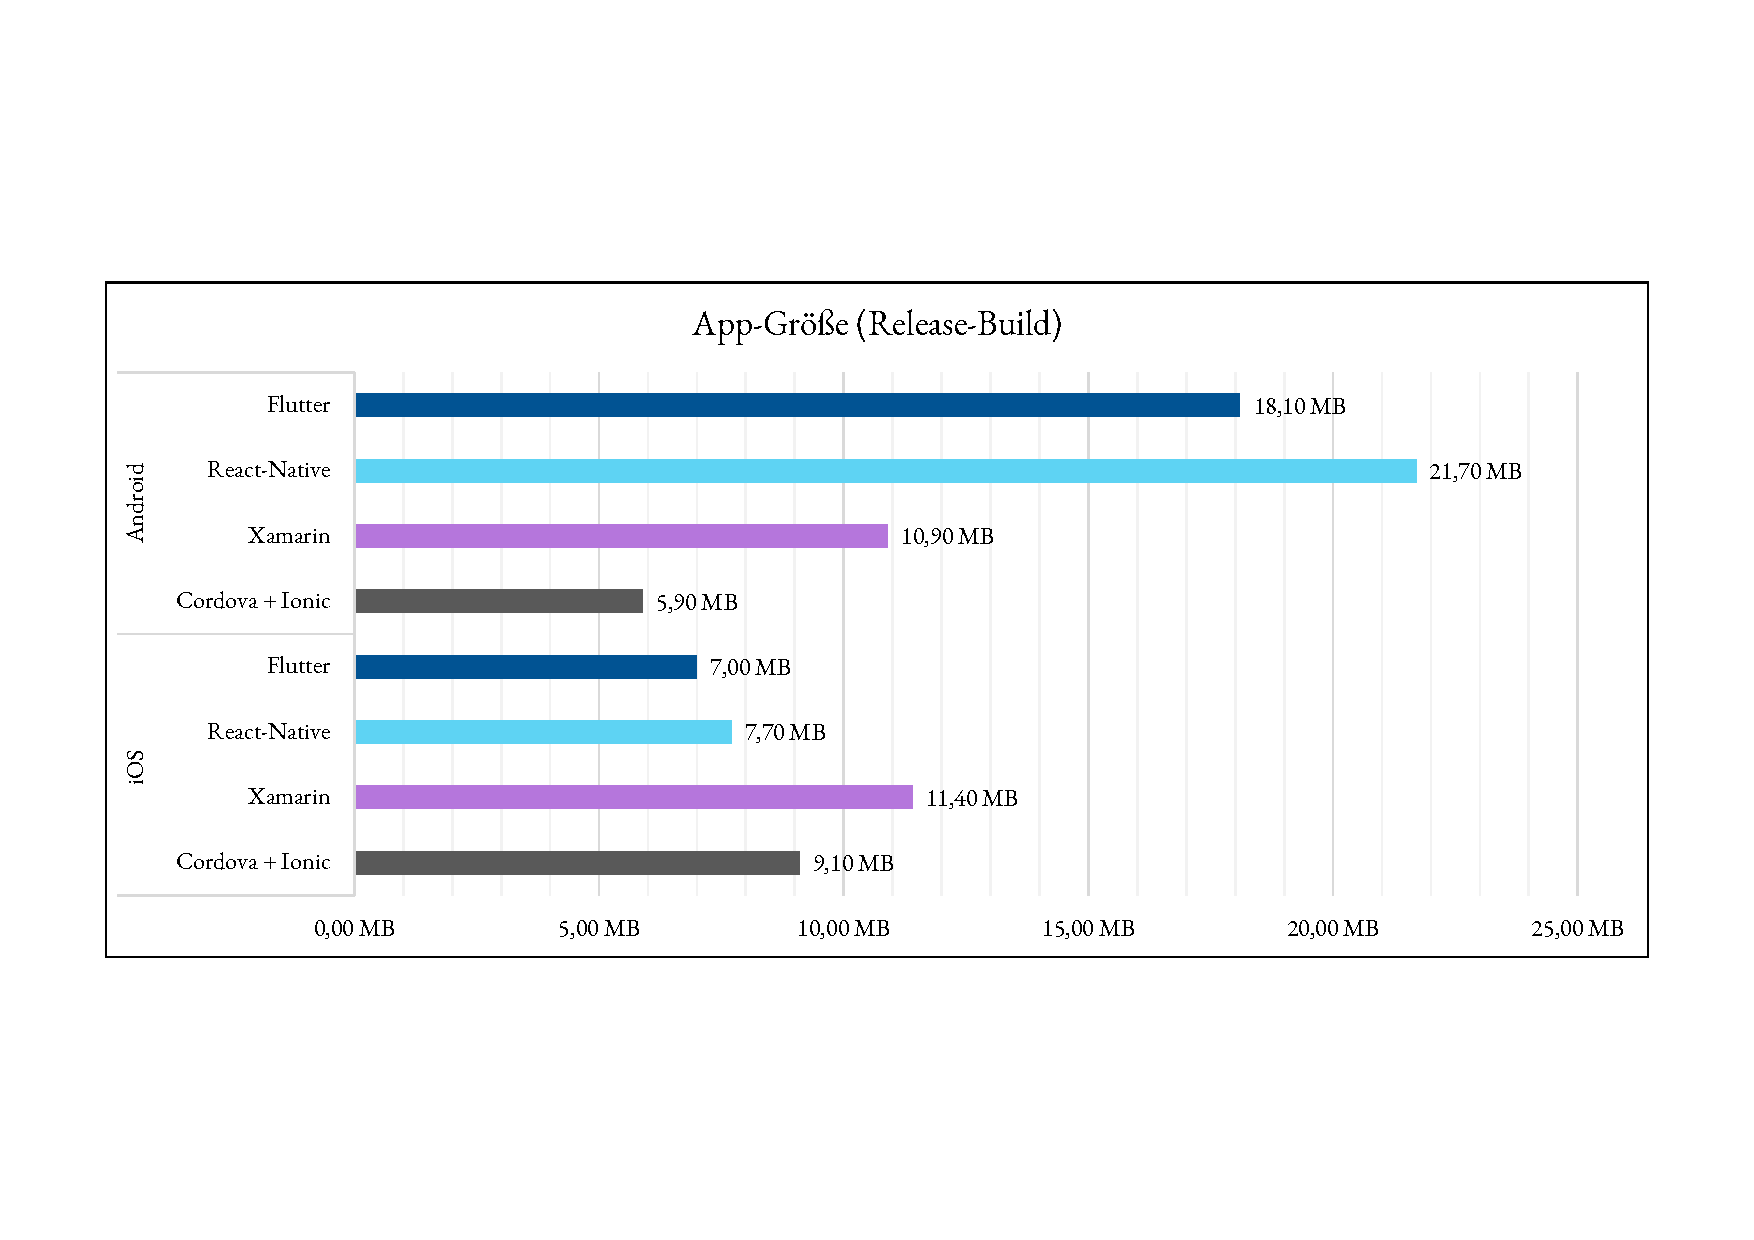
\includegraphics[trim=1.5cm 4.5cm 1.5cm 4.5cm, clip, width=0.9\textwidth]{app_size.pdf}
  \caption{Vergleich der Größe eines Release-Builds abhängig von Framework und Betriebssystem.}
  \label{fig:app_size}
\end{figure}

Unter Android sind die mit Ionic und Cordova und Xamarin erstellten Apps mit 5,9 MB und 10,9 MB die kleinsten.
Dies kann auf die Verwendung der vom Betriebssystem bereitgestellten Videoaufzeichnungsanwendung zurückgeführt werden.
Die Größe der App lässt sich reduzieren, indem die vom Betriebssystem bereitgestellte Anwendung aufgerufen wird, anstatt eine eigene Implementierung zu verwenden.
Die gleiche Argumentation lässt sich auch auf die jeweiligen Implementierungen für iOS übertragen.
Auch unter iOS ist die mit Ionic und Cordova erstellte App die kleinste.
Die Xamarin-Anwendung ist jedoch, wie durch die \ac{AOT}-Kompilation erwartet, unter iOS deutlich größer als unter Android.

Die mit Flutter und React Native erstellten Apps sind unter Android mit 18,1 MB und 21,7 MB deutlich größer als die mit Ionic und Cordova und Xamarin implementierten Anwendungen.
Dies lässt sich vermutlich auf die größere Menge der mitgelieferten Abhängigkeiten zurückführen.
Wie bei der Erläuterung der Frameworks in \autoref{sec:frameworks_flutter} beschrieben wird mit jeder Flutter-Anwendung eine Version der Skia Engine mitgeliefert.
Bei React Native muss jeweils eine JavaScript Engine mitgeliefert werden, in diesem Fall wird die für React Native optimierte Engine Hermes verwendet.
Beides führt zu im Vergleich zu anderen Frameworks größeren App-Bundles.
Jedoch ist die Flutter-Anwendung unter iOS nur minimal größer als unter Android und damit sehr konsistent über die Betriebssysteme hinweg.

Die mit React Native erstellte App ist unter iOS mit 157,6 MB deutlich größer ist als alle anderen Anwendungen unabhängig vom Betriebssystem.
Zwar ist die App unter Android ebenfalls größer als die anderen Anwendungen, jedoch ist der Unterschied deutlich geringer.
Sehr große \ac{IPA}-Dateien wurden bei der Verwendung der Hermes Engine bereits mehrfach beobachtet \cite{Hermes_appsize,Hermes_appsize_2}.
Wird anstatt Hermes, die von iOS bereitgestellte JavaScript Core Engine verwendet reduziert sich die App-Größe deutlich auf 3,1 MB, wie in \autoref{fig:reactnative_appsize_ios} zu sehen ist.
Unter Android trägt die Hermes Engine stattdessen zu einer kleineren App-Größe bei.
Ein Build mit der JavaScript Core Engine ist unter Android mit 51,9 MB deutlich größer als der Build mit der Hermes Engine mit 21,7 MB.
Da die Hermes Engine bei neuen React Native Projekten standardmäßig aktiviert ist, wird diese Variante für die Evaluation verwendet.
Außerdem ist anzumerken, dass die \ac{IPA}-Größe nicht repräsentativ für die Größe der App ist, welche über den App-Store verteilt wird.
Dies liegt daran, dass die \ac{IPA}-Datei verschiedene Varianten des Codes für verschiedene Geräte enthält und die finale, optimierte Version der App erst beim Upload zum App-Store erstellt wird \cite{IPA_Size}.
Da jedoch keine Methode bekannt ist, mit der die finale App-Größe bestimmt werden kann, ohne ein kostenpflichtiges Entwicklerkonto bei Apple zu besitzen, muss die \ac{IPA}-Größe zur Bewertung verwendet werden.

\begin{figure}[ht]
  \centering 
  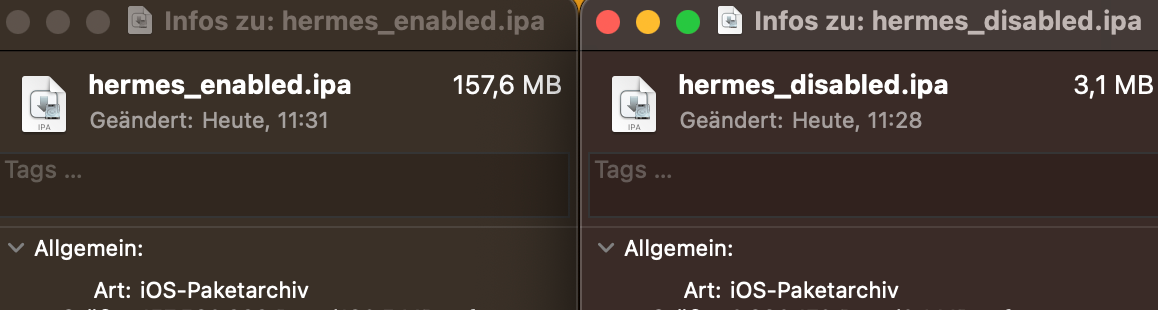
\includegraphics[clip, width=0.9\textwidth]{reactnative_appsize_ios}
   \caption{Vergleich der App-Größe einer React Native Anwendung für iOS mit und ohne Verwendung der Hermes Engine.}
  \label{fig:reactnative_appsize_ios}
\end{figure}


\subsection{Dauer bis zur vollständigen Funktionsfähigkeit}

Wie lange die jeweiligen Apps zwischen Start und vollständiger Funktionsfähigkeit benötigen, ist in \autoref{fig:launch_time} dargestellt.
Die Startzeiten wurden dabei fünfmal gemessen und ein Mittelwert gebildet.

Unter Android sind alle Startzeiten konsistent zwischen 50 und 64 \% schneller als unter iOS.
Die auf die durchschnittliche Startzeit auf dem jeweiligen Testgerät normalisierten Zeiten sind in \autoref{fig:launch_time_normalized} dargestellt.
Hier fallen kaum Unterschiede zwischen den Plattformen auf.
\begin{figure}[ht]
  \centering 
  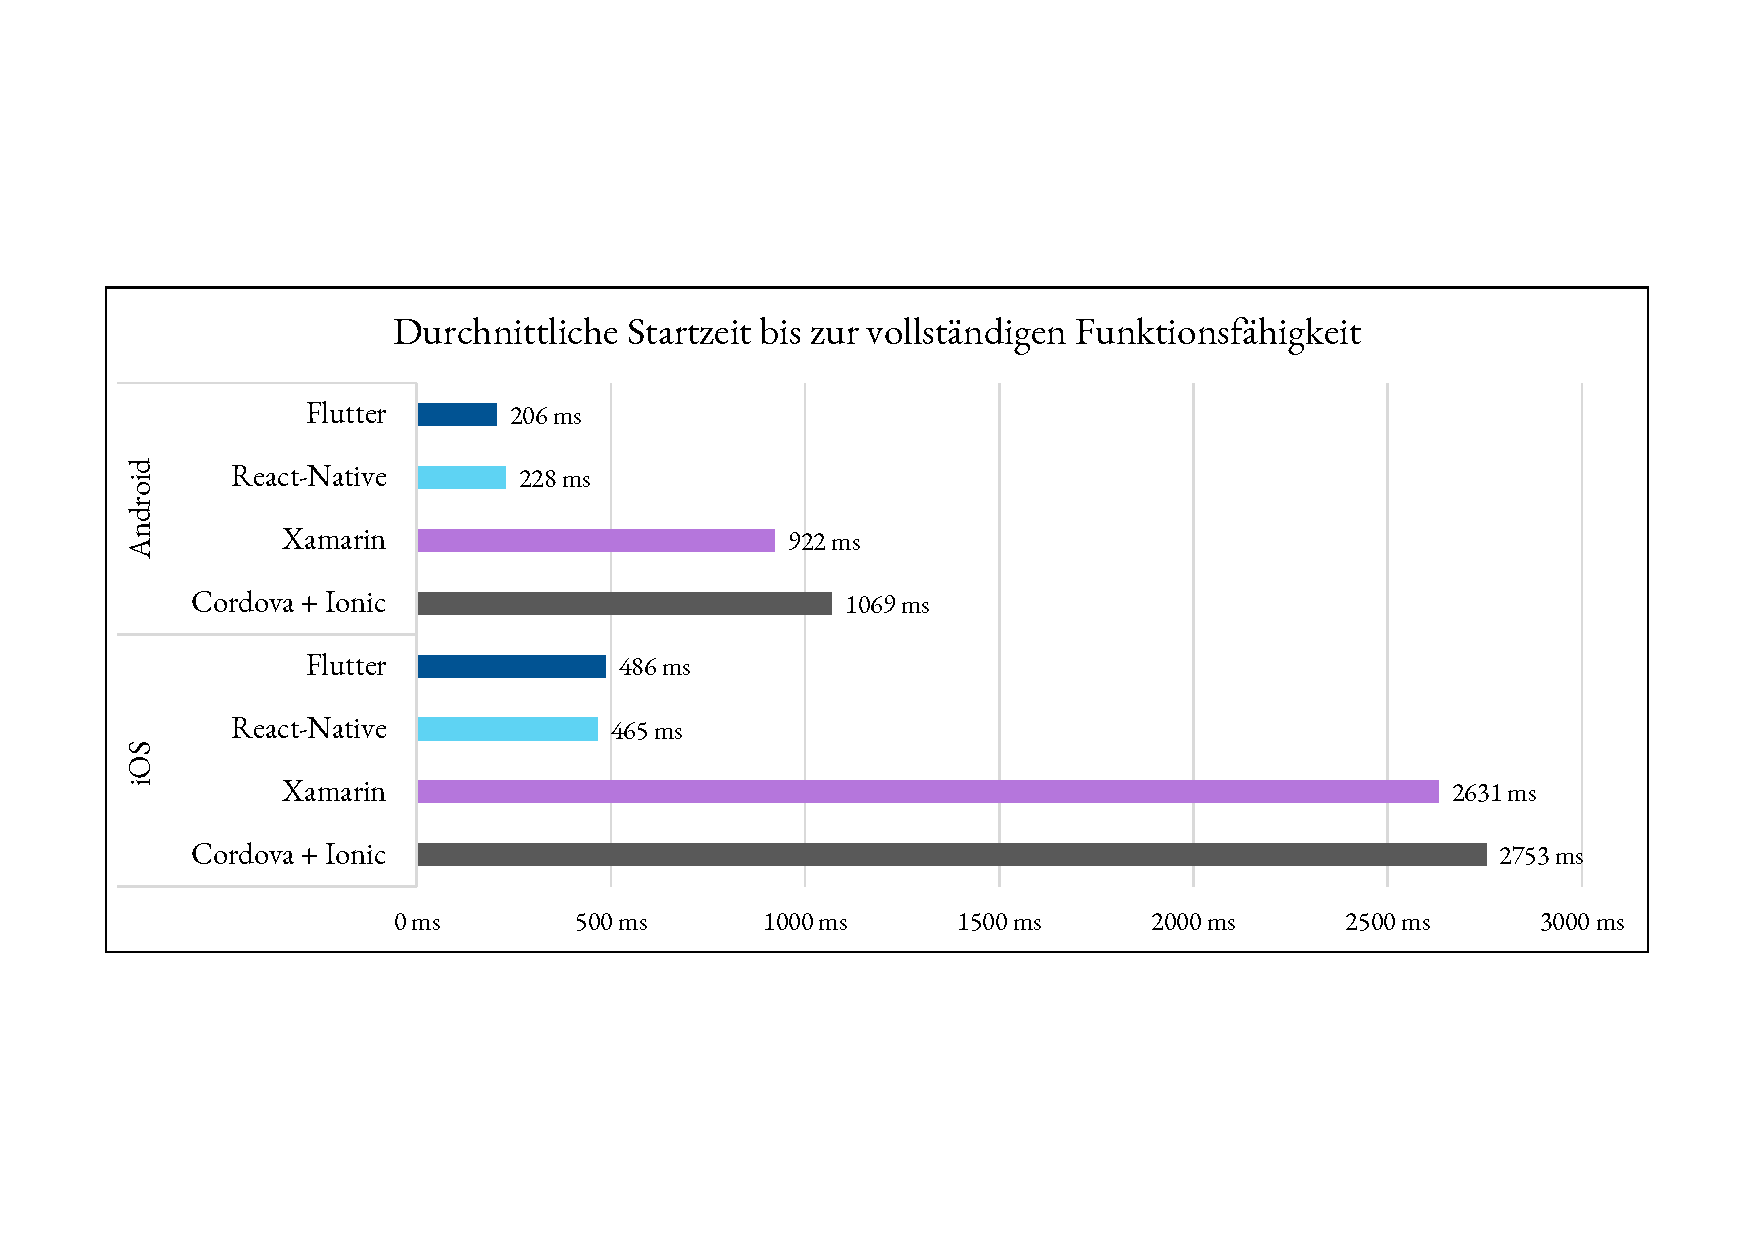
\includegraphics[trim=1.8cm 4.5cm 1.8cm 4.5cm, clip, width=0.9\textwidth]{launch_time.pdf}
  \caption{Vergleich der Zeit bis zur vollständigen Funktionsfähigkeit des Prototyps abhängig von Framework und Betriebssystem.}
  \label{fig:launch_time}
\end{figure}


Für die Messung der Startzeit kann bei Flutter und Xamarin auf die \ac{TTID} zurückgegriffen werden, die bei diesen Frameworks der Zeit bis zur vollständigen Funktionsfähigkeit entspricht.
Andererseits kann die \ac{TTID} bei React Native und Ionic mit Cordova nicht herangezogen werden, da diese Frameworks die Initialisierung nicht komplett abgeschlossen haben, wenn das erste Frame gerendert wird.
Bei Ionic mit Cordova wird stattdessen die Zeit bis zum Event \texttt{Platform.ready} gemessen, welches ausgelöst wird, sobald die Plattform bereit, also initialisiert ist.
Bei React Native wird die Zeit hingegen bis zum ersten Aufruf der Benutzerdefinierten \texttt{render}-Methode gemessen, da ab diesem Zeitpunkt beliebiger Code ausgeführt werden kann.
Von allen untersuchten Frameworks starten Flutter und React-Native Anwendungen am schnellsten.
Unter Android ist Flutter dabei etwas schneller als React Native, unter iOS ist es umgekehrt.
Trotz große konzeptueller Unterschiede zwischen den Frameworks ist eine ähnliche Startzeit erreichbar.

\begin{figure}[ht]
  \centering 
  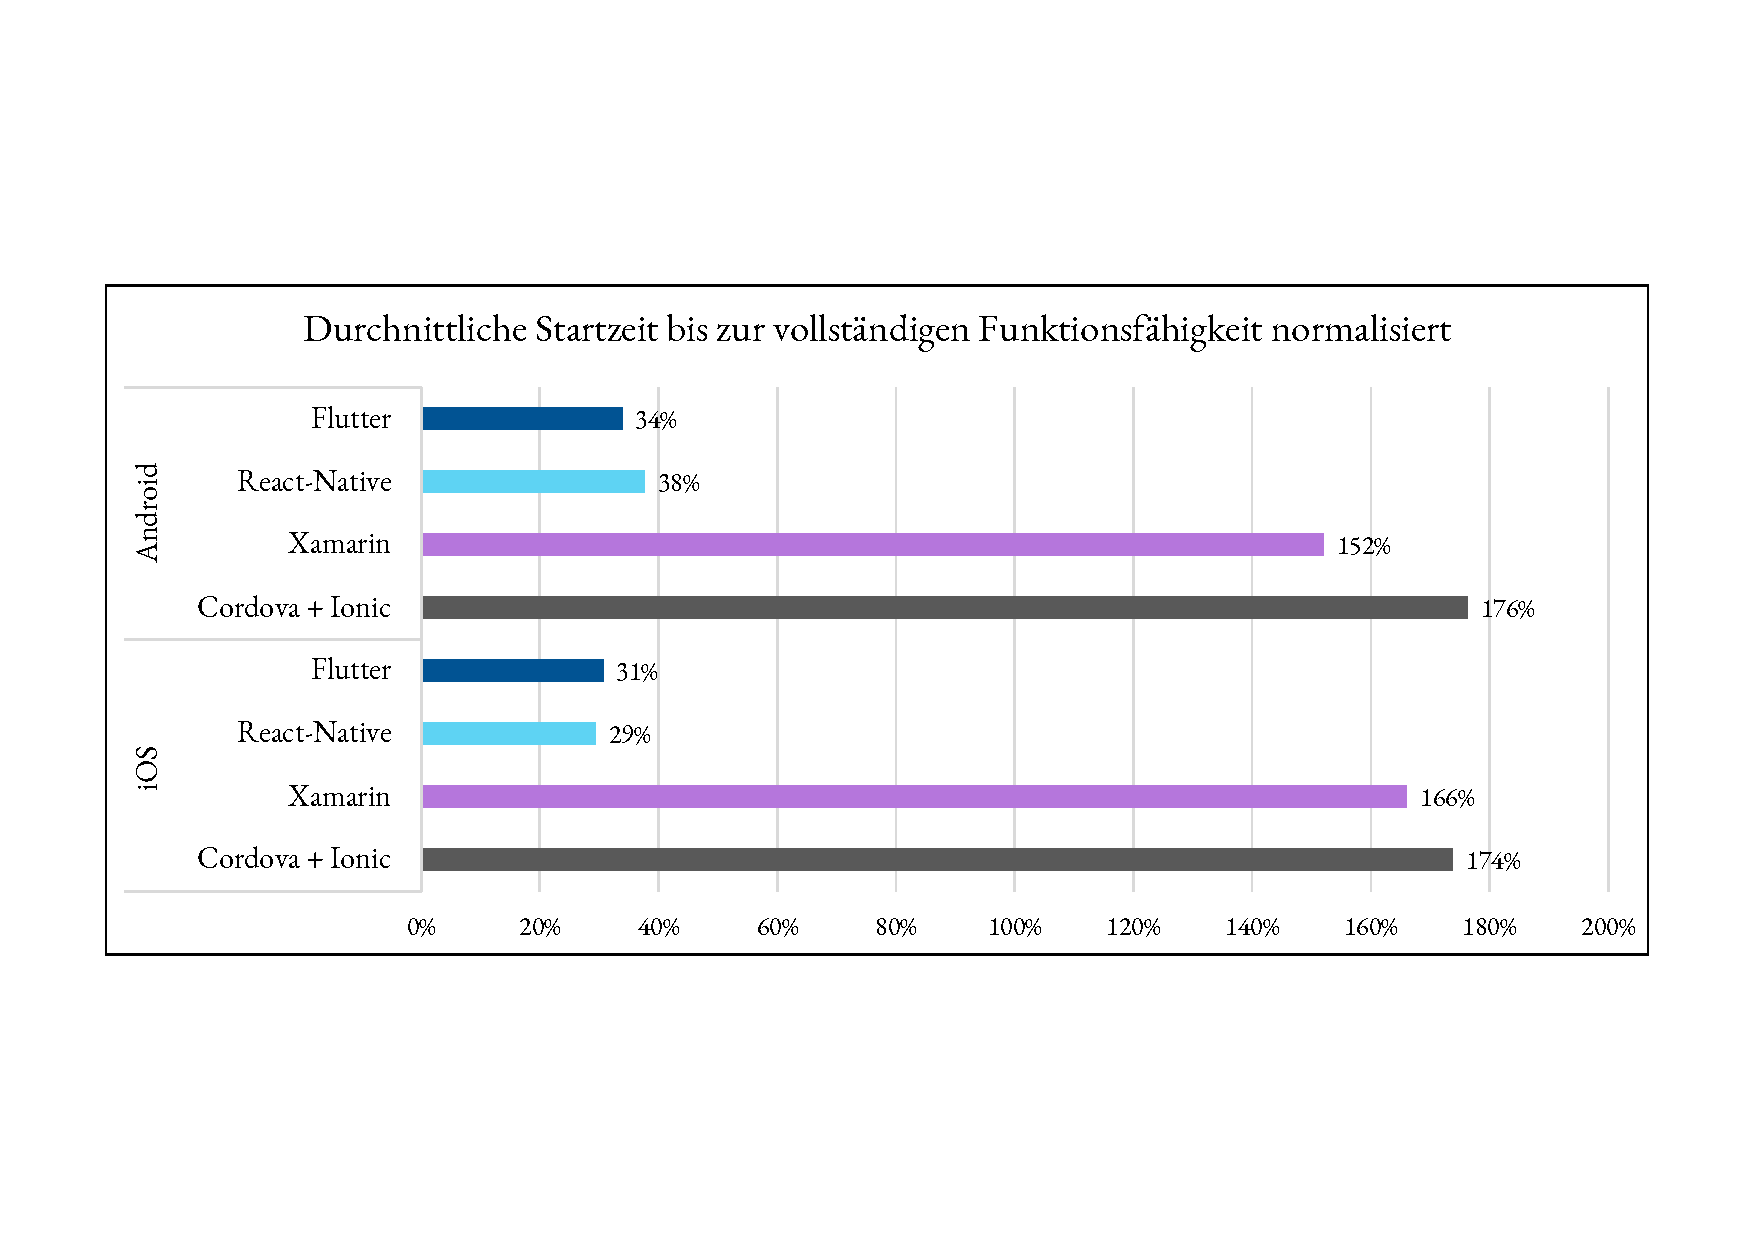
\includegraphics[trim=1.8cm 4.5cm 1.8cm 4.5cm, clip, width=0.9\textwidth]{launch_time_normalized.pdf}
  \caption{Vergleich der Zeit bis zur vollständigen Funktionsfähigkeit des Prototyps abhängig von Framework und Betriebssystem, normalisiert auf die durchschnittliche Startzeit des Geräts.}
  \label{fig:launch_time_normalized}
\end{figure}
Die Xamarin-Anwendung und die Anwendung, welche mit Ionic und Cordova implementiert ist, benötigen deutlich länger, bis die vollständige Funktionsfähigkeit erreicht ist.
Obwohl sowohl bei Ionic mit Cordova als auch bei React Native die Logik in JavaScript implementiert ist, ist die Startzeit der React Native-Anwendung mehr als viermal kürzer.
Daraus lässt sich schließen, dass der Ansatz von React Native, die nativen Steuerelemente der Plattform zu nutzen, anstatt eine WebView einzusetzen, beim Starten der Anwendung einen deutlichen Vorteil bietet.
Allerdings nutzt React Native auch eine für das Framework optimierte JavaScript Engine, was vermutlich ebenfalls einen positiven Einfluss auf die Startzeit hat.

Für Xamarin-Anwendungen wurde aufgrund der \ac{JIT}-Kompilation unter Android eine deutlich längere Startzeit als unter iOS erwartet.
Mit 166 \% der durchschnittlichen Startzeit unter iOS und 152 \% der durchschnittlichen Startzeit unter Android fällt der Unterschied zwischen den beiden Plattformen jedoch weniger stark aus als angenommen.
Ein Grund dafür konnte nicht identifiziert werden.
Zur besseren Vergleichbarkeit wäre es notwendig, die Startzeit auf beiden Plattformen mit der gleichen Hardware zu messen, was jedoch nicht möglich ist.

\subsection{Automatisierte Aufzeichnung und Speicherung eines zehnsekündigen Videos}

Die automatisierte Aufzeichnung und Speicherung von Videos ist nur bei Flutter- und React Native-Anwendungen möglich.
Sowohl bei Ionic mit Cordova als auch bei Xamarin kann die Aufzeichnung von Videos aufgrund der Verwendung der Standard-Videoaufzeichnungsanwendung nicht automatisiert werden.
Die in \autoref{fig:testcase} aufgeführten Zeiten, stellen jeweils einen Mittelwert aus fünf Messungen dar.
Für die Messung wurden dabei die von den Frameworks bereitgestellten Funktionen zur Zeitmessung verwendet.
Vom gemessenen Wert wird zusätzlich die Dauer des aufgezeichneten Videos abgezogen, da diese in allen Tests gleich gesetzt wurde.

\begin{figure}[ht]
  \centering 
  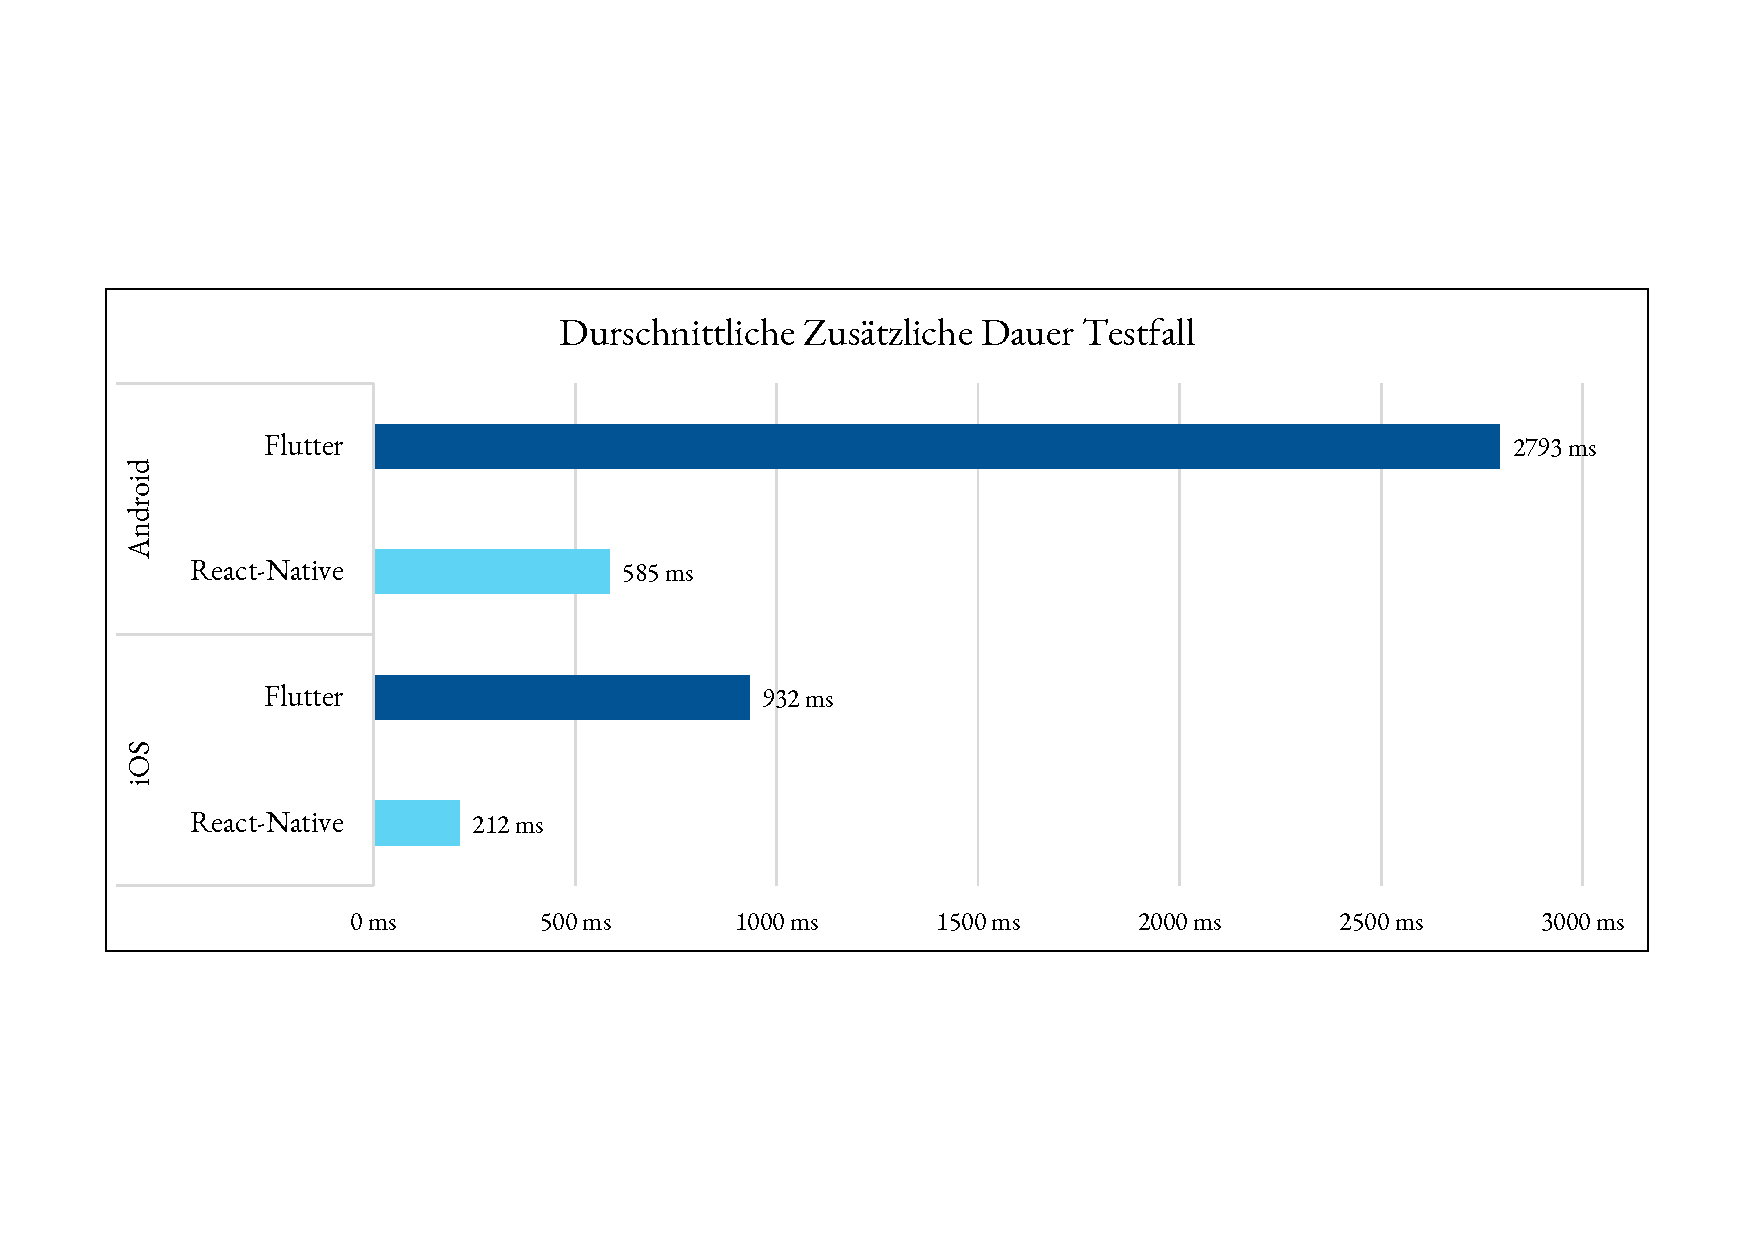
\includegraphics[trim=1.8cm 4.5cm 1.8cm 4.5cm, clip, width=0.9\textwidth]{testcase.pdf}
  \caption{Vergleich der für die Aufzeichnung und Speicherung von zehn Sekunden Video zusätzlich benötigten Zeit abhängig von Framework und Betriebssystem.}
  \label{fig:testcase}
\end{figure}

Direkt auffällig ist, dass die zusätzlich benötigte Zeit unter iOS deutlich geringer ausfällt als unter Android.
Dies lässt sich vermutlich darauf zurückführen, dass Aufzeichnung von Videos und Zugriff auf den Gerätespeicher unter iOS einen geringeren Overhead erzeugen als unter Android.
Allerdings müssen auch die Hardwareunterschiede betrachtet werden, sodass der direkte Vergleich nur bedingt aussagekräftig ist.

Die normalisierten Werte in \autoref{fig:testcase_normalized} zeigen, dass der Unterschied zwischen den Frameworks unter Android und iOS nahezu identisch ausfällt.
In beiden Fällen ist der automatisierte Testfall in der React Native-Anwendung mehr als viermal schneller als in der mit Flutter implementierten Anwendung.
Vermutlich ist die unterschiedliche Realisierung des Zugriffs auf nativen Code in den Frameworks verantwortlich für die beobachteten Performanceunterschiede.
\begin{figure}[ht]
  \centering 
  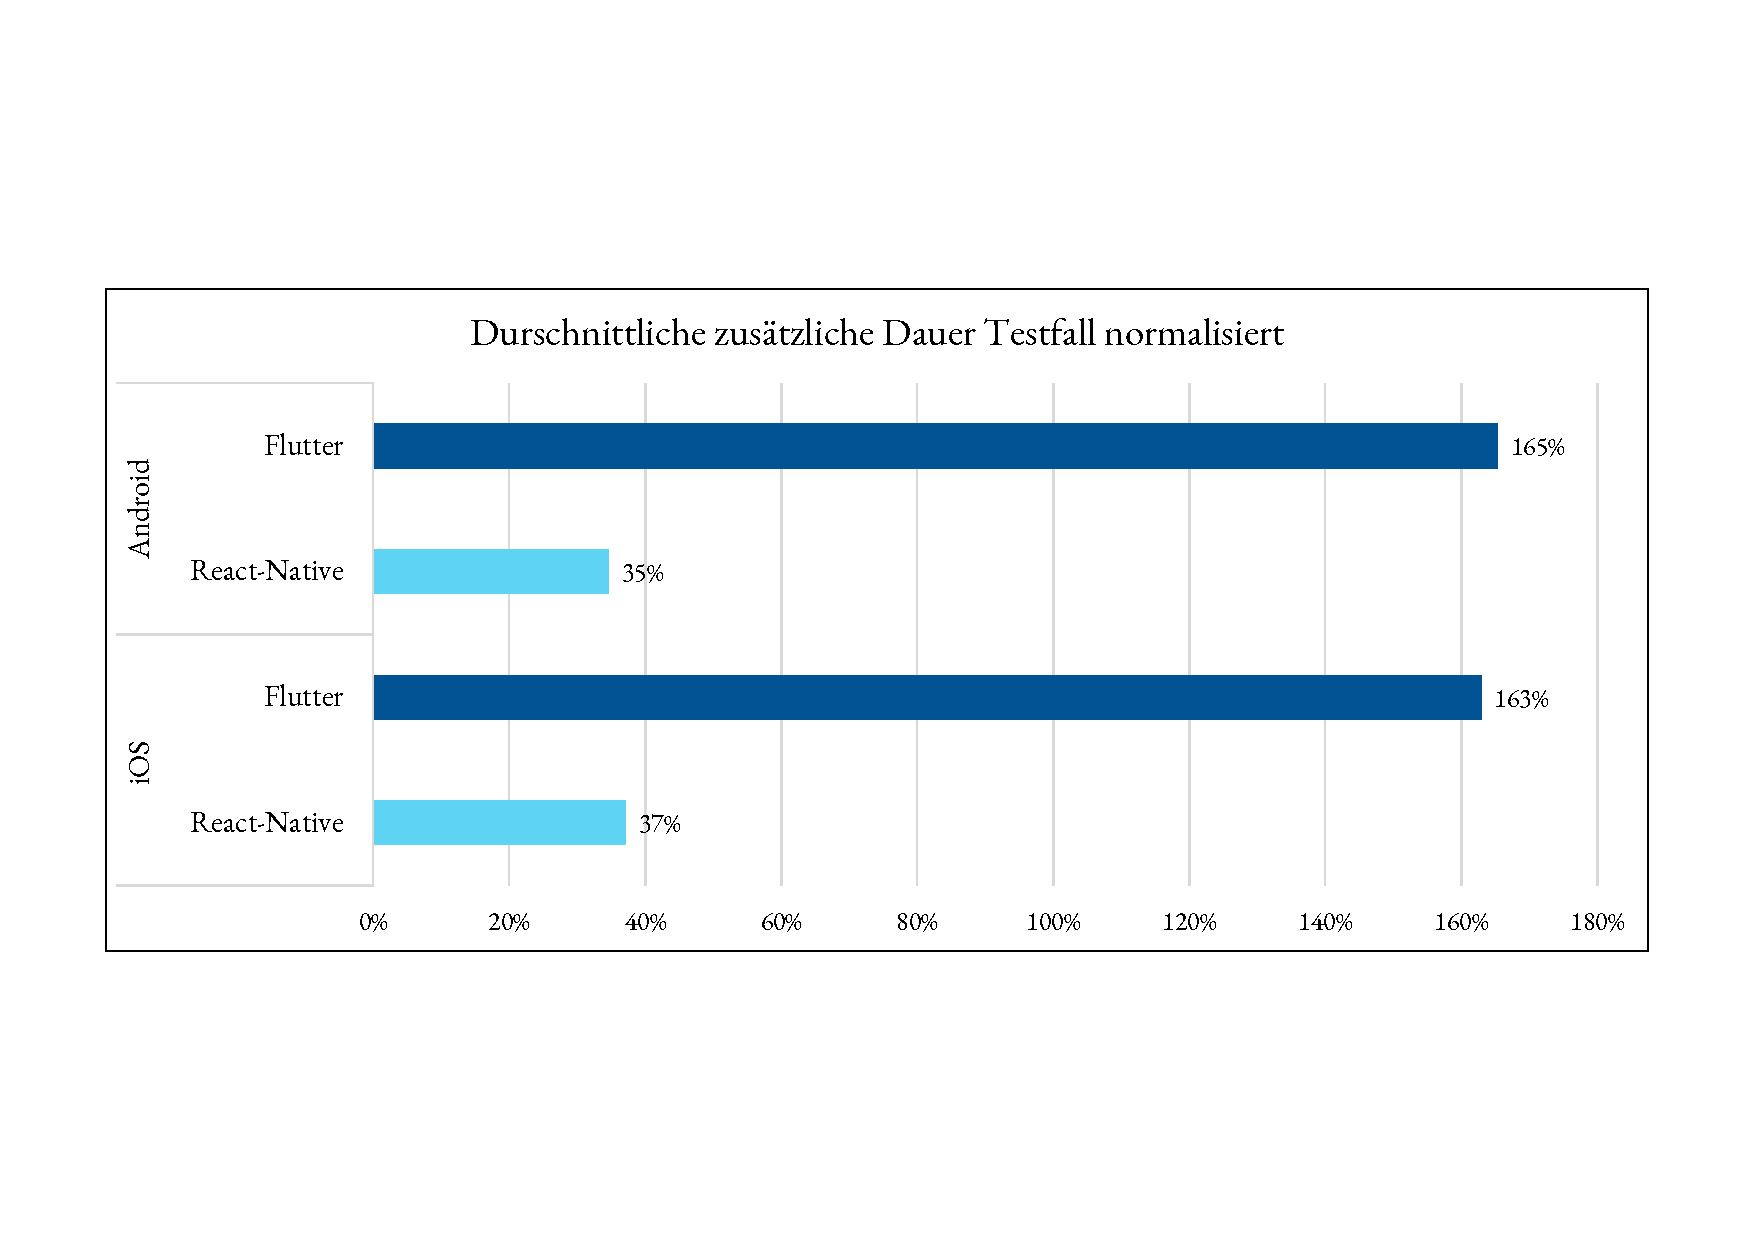
\includegraphics[trim=1.8cm 4.5cm 1.8cm 4.5cm, clip, width=0.9\textwidth]{testcase_normalized.pdf}
  \caption{Vergleich der für die Aufzeichnung und Speicherung von zehn Sekunden Video zusätzlich benötigten Zeit, normalisiert auf die durchschnittliche Zeit.}
  \label{fig:testcase_normalized}
\end{figure}

Das eingesetzte React Native Plugin verwendet die neue, in \autoref{sec:frameorks_reactnative} beschriebene, Architektur.
Damit können plattformspezifische Host-Objects direkt aus JavaScript aufgerufen werden, ohne dass eine Nachricht serialisiert und an eine native Implementierung übertragen werden muss.
Im Vergleich verwenden sowohl die alte Architektur von React Native als auch die Architektur von Flutter eine Nachrichtenbasierte Kommunikation.
Da das für React Native eingesetzte Plugin auf die neue Architektur angewiesen ist, ist kein direkter Vergleich zwischen neuer und alter Architektur möglich.
Es wird angenommen, dass die verwendete Architektur und das Kommunikationsmodell beim Zugriff auf native Funktionen die Unterschiede zwischen Flutter und React Native erklären.
Damit erlaubt React Native einen effizienteren Zugriff auf native Funktionalität, was nicht nur für Videoaufzeichnung, sondern auch für andere Funktionen gelten dürfte.